\providecommand{\Mod}{\mathbb{M}od}
\providecommand{\HomA}{\mathrm{Hom}_{A}}
\providecommand{\Fun}{\operatorname{Fun}}

\section{模的虚拟装备}\label{sec:virtual-equipment-of-modules}

\trInfinityCosmos{} $\mathcal{K}$ 中的模的\trVirtualDoubleCategory $\Mod(\mathcal{K})$ 具有%
刻画一个\emph{\trVirtualEquipment}（virtual equipment）的两个特殊性质。在陈述%
定义之前，我们先逐一考察它们。

\begin{proposition}[限制]\label{prop:restriction}
$\Mod(\mathcal{K})$ 中任何如下左图所示的图表皆可补全为一个\textbf{\trCartesian%
\trCell}（cartesian cell），如下右图所示
\begin{center}
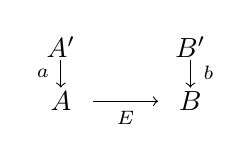
\begin{tikzpicture}[x=1.3em,y=1.3em]
  \node at (0,1.5) {$A'$};
  \node at (3.6,1.5) {$B'$};
  \node at (0,0) {$A$};
  \node at (3.6,0) {$B$};
  \draw[->] (0,1.15) -- (0,0.38);
  \node at (-0.5,0.78) {$\scriptstyle a$};
  \draw[->] (3.6,1.15) -- (3.6,0.38);
  \node at (4.1,0.78) {$\scriptstyle b$};
  \draw[->] (0.9,0) -- (2.7,0);
  \node at (1.8,-0.45) {$\scriptstyle E$};
\end{tikzpicture}
\qquad$\rightsquigarrow$\qquad
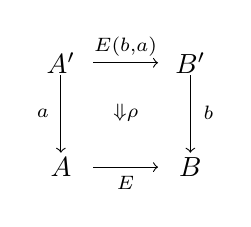
\begin{tikzpicture}[x=1.3em,y=1.3em]
  \node at (0,2.9) {$A'$};
  \node at (3.6,2.9) {$B'$};
  \node at (0,0) {$A$};
  \node at (3.6,0) {$B$};
  \draw[->] (0.9,2.9) -- (2.7,2.9);
  \node at (1.8,3.35) {$\scriptstyle E(b,a)$};
  \draw[->] (0,2.55) -- (0,0.4);
  \node at (-0.5,1.5) {$\scriptstyle a$};
  \draw[->] (3.6,2.55) -- (3.6,0.4);
  \node at (4.1,1.5) {$\scriptstyle b$};
  \node at (1.8,1.5) {$\scriptstyle\Downarrow\rho$};
  \draw[->] (0.9,0) -- (2.7,0);
  \node at (1.8,-0.45) {$\scriptstyle E$};
\end{tikzpicture}
\end{center}
并由如下\trUniversalProperty{}刻画：如下左图所示的任何胞腔都经由 $\rho$ 唯一地%
分解，如下右图所示：
\begin{center}
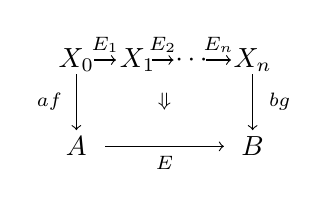
\begin{tikzpicture}[x=1.3em,y=1.3em]
  \node at (0,3) {$X_{0}$};
  \node at (1.7,3) {$X_{1}$};
  \node at (3.2,3) {$\cdots$};
  \node at (4.9,3) {$X_{n}$};
  \draw[->] (0.5,3) -- (1.1,3);
  \node at (0.8,3.42) {$\scriptstyle E_{1}$};
  \draw[->] (2.1,3) -- (2.7,3);
  \node at (2.4,3.42) {$\scriptstyle E_{2}$};
  \draw[->] (3.6,3) -- (4.3,3);
  \node at (3.95,3.42) {$\scriptstyle E_{n}$};
  \node at (0,0.6) {$A$};
  \node at (4.9,0.6) {$B$};
  \draw[->] (0,2.6) -- (0,1.05);
  \node at (-0.75,1.85) {$\scriptstyle af$};
  \draw[->] (4.9,2.6) -- (4.9,1.05);
  \node at (5.65,1.85) {$\scriptstyle bg$};
  \node at (2.45,1.85) {$\scriptstyle\Downarrow$};
  \draw[->] (0.8,0.6) -- (4.1,0.6);
  \node at (2.45,0.15) {$\scriptstyle E$};
\end{tikzpicture}
\qquad $:=$ \qquad
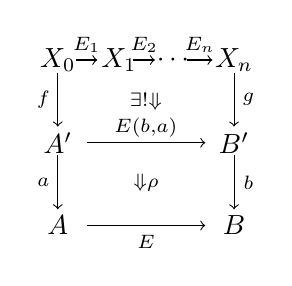
\begin{tikzpicture}[x=1.3em,y=1.3em]
  \node at (0,4.6) {$X_{0}$};
  \node at (1.7,4.6) {$X_{1}$};
  \node at (3.2,4.6) {$\cdots$};
  \node at (4.9,4.6) {$X_{n}$};
  \draw[->] (0.5,4.6) -- (1.1,4.6);
  \node at (0.8,5.02) {$\scriptstyle E_{1}$};
  \draw[->] (2.1,4.6) -- (2.7,4.6);
  \node at (2.4,5.02) {$\scriptstyle E_{2}$};
  \draw[->] (3.6,4.6) -- (4.3,4.6);
  \node at (3.95,5.02) {$\scriptstyle E_{n}$};
  \draw[->] (0,4.25) -- (0,2.75);
  \node at (-0.4,3.5) {$\scriptstyle f$};
  \node at (2.45,3.45) {$\scriptstyle\exists!\Downarrow$};
  \draw[->] (4.9,4.25) -- (4.9,2.75);
  \node at (5.3,3.5) {$\scriptstyle g$};
  \node at (0,2.3) {$A'$};
  \node at (4.9,2.3) {$B'$};
  \draw[->] (0.8,2.3) -- (4.1,2.3);
  \node at (2.45,2.72) {$\scriptstyle E(b,a)$};
  \draw[->] (0,1.95) -- (0,0.45);
  \node at (-0.4,1.2) {$\scriptstyle a$};
  \draw[->] (4.9,1.95) -- (4.9,0.45);
  \node at (5.3,1.2) {$\scriptstyle b$};
  \node at (2.45,1.2) {$\scriptstyle\Downarrow\rho$};
  \node at (0,0) {$A$};
  \node at (4.9,0) {$B$};
  \draw[->] (0.8,0) -- (4.1,0);
  \node at (2.45,-0.45) {$\scriptstyle E$};
\end{tikzpicture}
\end{center}
\end{proposition}

\begin{proof}
该\trCartesian\trCell{}的水平源由把模 $A\xrightarrow{E}B$ 沿函子 $a$ 与 $b$ 作%
限制而定义：
\begin{rveq}\label{eq:restriction-pullback}
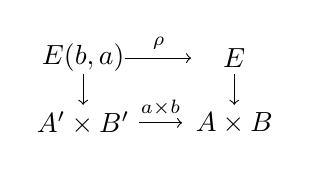
\begin{tikzpicture}[x=1.3em,y=1.3em]
  \node at (0,1.8) {$E(b,a)$};
  \node at (4.2,1.8) {$E$};
  \node at (0,0) {$A'\times B'$};
  \node at (4.2,0) {$A\times B$};
  \draw[->] (1.15,1.8) -- (3.0,1.8);
  \node at (2.1,2.22) {$\scriptstyle\rho$};
  \draw[->] (0,1.35) -- (0,0.5);
  \draw[->] (4.2,1.35) -- (4.2,0.5);
  \draw[->] (1.55,0) -- (2.75,0);
  \node at (2.15,0.42) {$\scriptstyle a\times b$};
  \node at (0.65,1.3) {$\scriptstyle\lrcorner$};
\end{tikzpicture}
\end{rveq}
由命题 7.4.5，这个左侧的\trIsofibration{}定义一个从 $A'$ 到 $B'$ 的\trModule{}；%
而由定义 8.1.4，其顶部的水平\trFunctor{}表示一个占据所求方块的\trModule{}映射。%
由观察 8.1.5，$\mathcal{K}$ 中的单纯\trPullback{}诱导\trFunctorSpace{}之间的%
如下\trEquivalence\footnote{若诸拉回按严格意义定义，则拉回事实上诱导%
\trFunctorSpace{}之间的一个\trIsomorphism；但即使把 $E(b,a)$ 换成一支等价的%
\trModule，诸\trFunctorSpace{}仍相等价，这已足以在对象的\trIsomorphism{}类上%
诱导一个双射。}
\begin{equation*}
\Fun_{f\times g}(E_{1}\times_{A_{1}}\cdots\times_{A_{n-1}}E_{n},\,E(b,a))
\xrightarrow[\ \simeq\ ]{\ \rho\circ-\ }
\Fun_{af\times bg}(E_{1}\times_{A_{1}}\cdots\times_{A_{n-1}}E_{n},\,E)
\end{equation*}
它在对象的\trIsomorphism{}类上下降为一个双射。这就给出了如上左图所示之胞腔%
经由笛卡尔的限制胞腔 $\rho$ 的唯一分解。
\end{proof}

我们把模 $A'\xrightarrow{E(b,a)}B'$ 称为模 $A\xrightarrow{E}B$ 沿函子 $a$ 与
$b$ 的\textbf{限制}（restriction），因为拉回 \eqref{eq:restriction-pullback}%
类似于双模沿一对环同态的\trRestrictionOfScalars。

\begin{example}\label{exa:hom-restriction}
模 $C\xrightarrow{\HomA(f,g)}B$ 是把由箭头 $\oo$-范畴
$A\overset{p_{1}}{\twoheadleftarrow}A^{2}\overset{p_{0}}{\twoheadrightarrow}A$
所编码的模沿 $g\colon C\to A$ 与 $f\colon B\to A$ 作限制的结果。为使这一限制%
关系更加透明，当把箭头 $\oo$-范畴视为一个\trModule{}时，我们通常把它写作
$A\xrightarrow{\HomA}A$。
\begin{center}
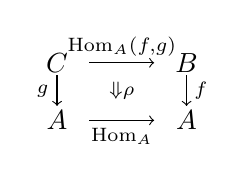
\begin{tikzpicture}[x=1.3em,y=1.3em]
  \node at (0,1.6) {$C$};
  \node at (3.6,1.6) {$B$};
  \node at (0,0) {$A$};
  \node at (3.6,0) {$A$};
  \draw[->] (0.9,1.6) -- (2.7,1.6);
  \node at (1.8,2.05) {$\scriptstyle\HomA(f,g)$};
  \draw[->] (0,1.25) -- (0,0.4);
  \node at (-0.4,0.82) {$\scriptstyle g$};
  \draw[->] (3.6,1.25) -- (3.6,0.4);
  \node at (4.0,0.82) {$\scriptstyle f$};
  \node at (1.8,0.82) {$\scriptstyle\Downarrow\rho$};
  \draw[->] (0.9,0) -- (2.7,0);
  \node at (1.8,-0.45) {$\scriptstyle\HomA$};
\end{tikzpicture}
\end{center}
由于 hom \trBifunctor{}的通行记法把逆变变元置于左侧、把协变变元置于右侧，我们在%
\cref{prop:restriction}中对限制采用了类似的记号约定。
\end{example}

\begin{proposition}[单位]\label{prop:units}
$\Mod(\mathcal{K})$ 中的任何对象 $A$ 都配备有一个零元\textbf{\trCocartesian%
\trCell}（cocartesian cell）
\begin{center}
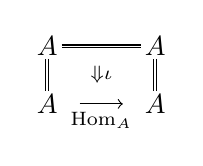
\begin{tikzpicture}[x=1.3em,y=1.3em]
  \node at (0,1.6) {$A$};
  \node at (3.0,1.6) {$A$};
  \node at (0,0) {$A$};
  \node at (3.0,0) {$A$};
  \draw[double,double distance=0.6pt] (0.4,1.6) -- (2.6,1.6);
  \draw[double,double distance=0.6pt] (0,1.25) -- (0,0.35);
  \draw[double,double distance=0.6pt] (3.0,1.25) -- (3.0,0.35);
  \node at (1.5,0.8) {$\scriptstyle\Downarrow\iota$};
  \draw[->] (0.9,0) -- (2.1,0);
  \node at (1.5,-0.45) {$\scriptstyle\HomA$};
\end{tikzpicture}
\end{center}
并由如下\trUniversalProperty{}刻画：$\Mod(\mathcal{K})$ 中任何水平源包含对象
$A$ 的胞腔都经由 $\iota$ 唯一地分解，如下所示：
\begin{center}
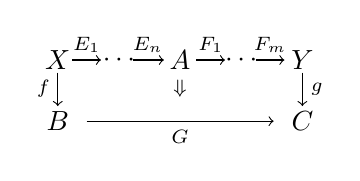
\begin{tikzpicture}[x=1.3em,y=1.3em]
  \node at (0,1.7) {$X$};
  \node at (1.7,1.7) {$\cdots$};
  \node at (3.4,1.7) {$A$};
  \node at (5.1,1.7) {$\cdots$};
  \node at (6.8,1.7) {$Y$};
  \draw[->] (0.4,1.7) -- (1.2,1.7);
  \node at (0.8,2.12) {$\scriptstyle E_{1}$};
  \draw[->] (2.1,1.7) -- (2.95,1.7);
  \node at (2.5,2.12) {$\scriptstyle E_{n}$};
  \draw[->] (3.85,1.7) -- (4.65,1.7);
  \node at (4.25,2.12) {$\scriptstyle F_{1}$};
  \draw[->] (5.5,1.7) -- (6.3,1.7);
  \node at (5.9,2.12) {$\scriptstyle F_{m}$};
  \draw[->] (0,1.35) -- (0,0.42);
  \node at (-0.4,0.9) {$\scriptstyle f$};
  \draw[->] (6.8,1.35) -- (6.8,0.42);
  \node at (7.2,0.9) {$\scriptstyle g$};
  \node at (3.4,0.9) {$\scriptstyle\Downarrow$};
  \node at (0,0) {$B$};
  \node at (6.8,0) {$C$};
  \draw[->] (0.8,0) -- (6.0,0);
  \node at (3.4,-0.45) {$\scriptstyle G$};
\end{tikzpicture}
\qquad $:=$
\end{center}
\begin{center}
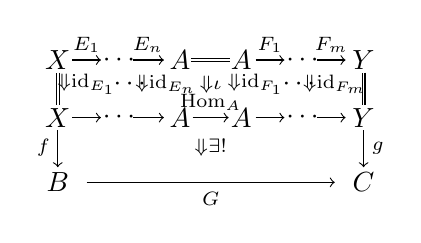
\begin{tikzpicture}[x=1.3em,y=1.3em]
  \node at (0,3.4) {$X$};
  \node at (1.7,3.4) {$\cdots$};
  \node at (3.4,3.4) {$A$};
  \node at (5.1,3.4) {$A$};
  \node at (6.8,3.4) {$\cdots$};
  \node at (8.5,3.4) {$Y$};
  \draw[->] (0.4,3.4) -- (1.2,3.4);
  \node at (0.8,3.82) {$\scriptstyle E_{1}$};
  \draw[->] (2.1,3.4) -- (2.95,3.4);
  \node at (2.5,3.82) {$\scriptstyle E_{n}$};
  \draw[double,double distance=0.6pt] (3.7,3.4) -- (4.8,3.4);
  \draw[->] (5.5,3.4) -- (6.3,3.4);
  \node at (5.9,3.82) {$\scriptstyle F_{1}$};
  \draw[->] (7.2,3.4) -- (8.0,3.4);
  \node at (7.6,3.82) {$\scriptstyle F_{m}$};
  \draw[double,double distance=0.6pt] (0,3.05) -- (0,2.15);
  \draw[double,double distance=0.6pt] (8.5,3.05) -- (8.5,2.15);
  \node at (0.8,2.72) {$\scriptstyle\Downarrow\mathrm{id}_{E_{1}}$};
  \node at (2.0,2.72) {$\cdots$};
  \node at (3.0,2.72) {$\scriptstyle\Downarrow\mathrm{id}_{E_{n}}$};
  \node at (4.25,2.72) {$\scriptstyle\Downarrow\iota$};
  \node at (5.5,2.72) {$\scriptstyle\Downarrow\mathrm{id}_{F_{1}}$};
  \node at (6.7,2.72) {$\cdots$};
  \node at (7.7,2.72) {$\scriptstyle\Downarrow\mathrm{id}_{F_{m}}$};
  \node at (0,1.8) {$X$};
  \node at (1.7,1.8) {$\cdots$};
  \node at (3.4,1.8) {$A$};
  \node at (5.1,1.8) {$A$};
  \node at (6.8,1.8) {$\cdots$};
  \node at (8.5,1.8) {$Y$};
  \draw[->] (0.4,1.8) -- (1.2,1.8);
  \draw[->] (2.1,1.8) -- (2.95,1.8);
  \draw[->] (3.75,1.8) -- (4.75,1.8);
  \node at (4.25,2.22) {$\scriptstyle\HomA$};
  \draw[->] (5.5,1.8) -- (6.3,1.8);
  \draw[->] (7.2,1.8) -- (8.0,1.8);
  \draw[->] (0,1.45) -- (0,0.42);
  \node at (-0.4,0.95) {$\scriptstyle f$};
  \draw[->] (8.5,1.45) -- (8.5,0.42);
  \node at (8.9,0.95) {$\scriptstyle g$};
  \node at (4.25,0.95) {$\scriptstyle\Downarrow\exists!$};
  \node at (0,0) {$B$};
  \node at (8.5,0) {$C$};
  \draw[->] (0.8,0) -- (7.7,0);
  \node at (4.25,-0.45) {$\scriptstyle G$};
\end{tikzpicture}
\end{center}
\end{proposition}

\begin{proof}
该零元胞腔由 $A$ 处的恒同 $1$-胞腔上的恒同 $2$-胞腔所诱导的\trSpan{}映射表示：
\begin{center}
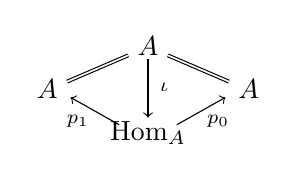
\begin{tikzpicture}[x=1.3em,y=1.3em]
  \node at (0,2.4) {$A$};
  \node at (-2.8,1.2) {$A$};
  \node at (2.8,1.2) {$A$};
  \node at (0,0) {$\HomA$};
  \draw[double,double distance=0.6pt] (-0.55,2.15) -- (-2.25,1.42);
  \draw[double,double distance=0.6pt] (0.55,2.15) -- (2.25,1.42);
  \draw[->] (0,2.05) -- (0,0.42);
  \node at (0.45,1.25) {$\scriptstyle\iota$};
  \draw[->] (-0.8,0.22) -- (-2.15,0.98);
  \node at (-1.95,0.32) {$\scriptstyle p_{1}$};
  \draw[->] (0.8,0.22) -- (2.15,0.98);
  \node at (1.95,0.32) {$\scriptstyle p_{0}$};
\end{tikzpicture}
\qquad $\mathrel{\leftrightsquigarrow}$ \qquad
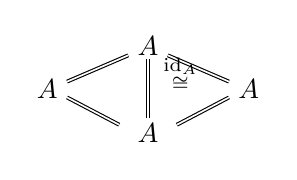
\begin{tikzpicture}[x=1.3em,y=1.3em]
  \node at (0,2.4) {$A$};
  \node at (-2.8,1.2) {$A$};
  \node at (2.8,1.2) {$A$};
  \node at (0,0) {$A$};
  \draw[double,double distance=0.6pt] (-0.55,2.15) -- (-2.25,1.42);
  \draw[double,double distance=0.6pt] (0.55,2.15) -- (2.25,1.42);
  \draw[double,double distance=0.6pt] (-2.25,0.98) -- (-0.8,0.22);
  \draw[double,double distance=0.6pt] (2.25,0.98) -- (0.8,0.22);
  \draw[double,double distance=0.6pt] (0,2.05) -- (0,0.42);
  \node at (0.9,1.85) {$\scriptstyle\mathrm{id}_{A}$};
  \node at (0.9,1.35) {$\scriptstyle\cong$};
\end{tikzpicture}
\end{center}
在别处，这个\trFunctor{}记作
$\ulcorner\mathrm{id}_{A}\urcorner\colon A\to A^{2}$；回忆%
\cref{exa:hom-restriction}：我们把箭头 $\oo$-范畴构造所编码的模写作
$A\xrightarrow{\HomA}A$，正是为了帮助我们识别它的诸限制。

在序列 $E_{i}$ 与 $F_{j}$ 皆为空的情形，由定理 7.4.8 给出的模的\trYonedaLemma{}%
的单侧版本告诉我们：沿这一映射的限制诱导\trFunctorSpace{}的一个\trEquivalence
\begin{equation*}
\Fun_{A\times A}(\HomA,G(g,f))
\Rightarrow
\Fun_{A\times A}(A,G(g,f)).
\end{equation*}
取对象的\trIsomorphism{}类即得该陈述中的双射。

在序列之一或两者皆非空的情形，我们可以作出把它们水平复合而成的%
\trTwoSidedFibration{} $X\xleftarrow{q}E\xrightarrow{p}A$ 与
$A\xleftarrow{s}F\xrightarrow{r}Y$，然后对如下可复合三元组作出水平复合
$E\times_{A}\HomA$ 或水平复合 $\HomA\times_{A}F$：
\begin{center}
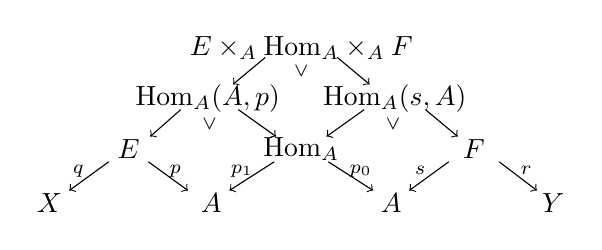
\begin{tikzpicture}[x=1.3em,y=1.3em]
  \node at (2.6,4.3) {$E\times_{A}\HomA\times_{A}F$};
  \node at (0,2.9) {$\HomA(A,p)$};
  \node at (5.2,2.9) {$\HomA(s,A)$};
  \node at (-2.2,1.5) {$E$};
  \node at (2.6,1.5) {$\HomA$};
  \node at (7.4,1.5) {$F$};
  \node at (-4.4,0) {$X$};
  \node at (0.1,0) {$A$};
  \node at (5.1,0) {$A$};
  \node at (9.6,0) {$Y$};
  \draw[->] (1.6,4.05) -- (0.7,3.3);
  \draw[->] (3.6,4.05) -- (4.5,3.3);
  \node at (2.6,3.68) {$\scriptstyle\vee$};
  \draw[->] (-0.75,2.6) -- (-1.6,1.85);
  \draw[->] (0.85,2.6) -- (1.9,1.85);
  \node at (0.05,2.2) {$\scriptstyle\vee$};
  \draw[->] (4.35,2.6) -- (3.3,1.85);
  \draw[->] (6.05,2.6) -- (6.95,1.85);
  \node at (5.15,2.2) {$\scriptstyle\vee$};
  \draw[->] (-2.75,1.15) -- (-3.85,0.35);
  \node at (-3.6,0.9) {$\scriptstyle q$};
  \draw[->] (-1.65,1.15) -- (-0.55,0.35);
  \node at (-0.9,0.9) {$\scriptstyle p$};
  \draw[->] (1.85,1.15) -- (0.6,0.35);
  \node at (0.95,0.9) {$\scriptstyle p_{1}$};
  \draw[->] (3.35,1.15) -- (4.6,0.35);
  \node at (4.25,0.9) {$\scriptstyle p_{0}$};
  \draw[->] (6.7,1.15) -- (5.6,0.35);
  \node at (5.9,0.9) {$\scriptstyle s$};
  \draw[->] (8.1,1.15) -- (9.15,0.35);
  \node at (8.85,0.9) {$\scriptstyle r$};
\end{tikzpicture}
\end{center}
左边那一对\trModule{}的水平复合是\trTwoSidedFibration{}
$(qp_{1},p_{0})\colon\HomA(A,p)\twoheadrightarrow X\times A$，而右边那一对的%
复合是\trTwoSidedFibration{}
$(p_{1},rp_{0})\colon\HomA(s,A)\twoheadrightarrow A\times Y$。由定理 7.1.4，%
这些\trTwoSidedFibration{}给出如下\trFiberedAdjunction：
\begin{center}
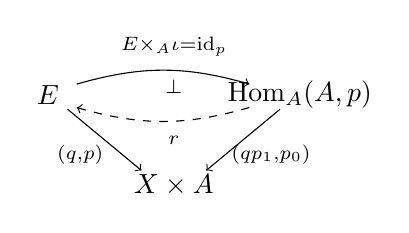
\begin{tikzpicture}[x=1.3em,y=1.3em]
  \node at (0,1.4) {$E$};
  \node at (7.0,1.4) {$\HomA(A,p)$};
  \node at (3.5,-1.1) {$X\times A$};
  \draw[->] (0.8,1.7) to[bend left=16] (5.6,1.7);
  \node at (3.5,2.75) {$\scriptstyle E\times_{A}\iota=\ulcorner\mathrm{id}_{p}\urcorner$};
  \node at (3.5,1.62) {$\scriptstyle\perp$};
  \draw[->,dashed] (5.6,1.05) to[bend left=16] (0.8,1.05);
  \node at (3.5,0.15) {$\scriptstyle r$};
  \draw[->] (0.55,1.0) -- (2.6,-0.7);
  \node at (0.9,-0.25) {$\scriptstyle(q,p)$};
  \draw[->] (6.45,1.0) -- (4.4,-0.7);
  \node at (6.2,-0.25) {$\scriptstyle(qp_{1},p_{0})$};
\end{tikzpicture}
\qquad
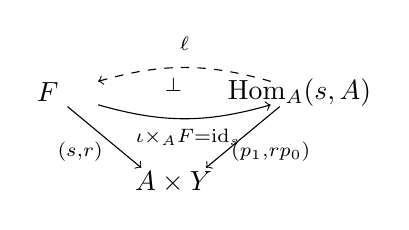
\begin{tikzpicture}[x=1.3em,y=1.3em]
  \node at (0,1.4) {$F$};
  \node at (7.0,1.4) {$\HomA(s,A)$};
  \node at (3.5,-1.1) {$A\times Y$};
  \draw[->,dashed] (6.2,1.7) to[bend right=16] (1.4,1.7);
  \node at (3.8,2.75) {$\scriptstyle\ell$};
  \node at (3.5,1.62) {$\scriptstyle\perp$};
  \draw[->] (1.4,1.05) to[bend right=16] (6.2,1.05);
  \node at (3.9,0.15) {$\scriptstyle\iota\times_{A}F=\ulcorner\mathrm{id}_{s}\urcorner$};
  \draw[->] (0.55,1.0) -- (2.6,-0.7);
  \node at (0.9,-0.25) {$\scriptstyle(s,r)$};
  \draw[->] (6.45,1.0) -- (4.4,-0.7);
  \node at (6.2,-0.25) {$\scriptstyle(p_{1},rp_{0})$};
\end{tikzpicture}
\end{center}

经直接观察，实线箭头的两根伴随 $\ulcorner\mathrm{id}_{p}\urcorner$ 与
$\ulcorner\mathrm{id}_{s}\urcorner$ 可以通过拉回映射 $\iota\colon A\to\HomA$ 而%
构造。

我们只需要其中一个伴随，故不失一般性地取前者。这一\trFiberedAdjunction{}沿 $s$ 拉回、沿 $r$
前推，定义出\trTwoSidedFibration{}之间的如下\trFiberedAdjunction
\begin{center}
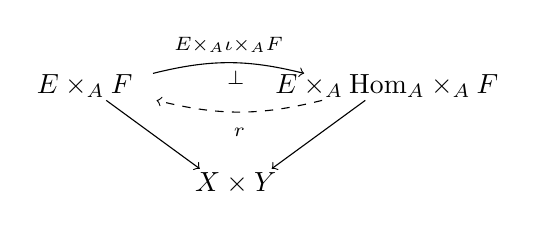
\begin{tikzpicture}[x=1.3em,y=1.3em]
  \node at (0,1.5) {$E\times_{A}F$};
  \node at (8.4,1.5) {$E\times_{A}\HomA\times_{A}F$};
  \node at (4.2,-1.2) {$X\times Y$};
  \draw[->] (1.9,1.85) to[bend left=14] node[above,pos=0.5]{$\scriptstyle E\times_{A}\iota\times_{A}F$} (6.1,1.85);
  \node at (4.2,1.72) {$\scriptstyle\perp$};
  \draw[->,dashed] (6.6,1.1) to[bend left=14] (2.0,1.1);
  \node at (4.3,0.2) {$\scriptstyle r$};
  \draw[->] (0.6,1.1) -- (3.2,-0.8);
  \draw[->] (7.8,1.1) -- (5.2,-0.8);
\end{tikzpicture}
\end{center}
当映入 $\mathcal{K}_{/X\times Y}$ 中的\trDiscrete{}对象 $G(g,f)$ 时，这一伴随%
成为一个\trAdjointEquivalence{}。特别地，沿 $\iota$ 的限制诱导\trKanComplex{}之间%
的一个\trEquivalence
\begin{equation*}
\Fun_{X\times Y}(E\times_{A}\HomA\times_{A}F,\,G(g,f))
\xrightarrow[\ \simeq\ ]{\ -\circ(E\times_{A}\iota\times_{A}F)\ }
\Fun_{X\times Y}(E\times_{A}F,\,G(g,f)),
\end{equation*}
而再一次取对象的\trIsomorphism{}类即给出该陈述中的双射。
\end{proof}

\cref{prop:restriction}与\cref{prop:units}蕴含：模的\trVirtualDoubleCategory{}是 Cruttwell 与
Shulman（\cite{bib32}，第 7 节）所引入意义下的一个\emph{\trVirtualEquipment}。

\begin{definition}\label{def:virtual-equipment}
一个\textbf{\trVirtualEquipment}是一个满足如下条件的\trVirtualDoubleCategory{}：
\begin{enumerate}[label=(\roman*)]
\item 对任何水平箭头 $A\xrightarrow{E}B$ 与任何一对竖直箭头
$a\colon A'\to A$ 和 $b\colon B'\to B$，都存在一个水平箭头
$A'\xrightarrow{E(b,a)}B'$\footnote{原书印作「$B'\xrightarrow{E(b,a)}A'$」。
按\cref{prop:restriction}，限制 $E(b,a)$ 是从 $A'$ 到 $B'$ 的\trModule{}（该
命题图示顶行即 $A'\xrightarrow{E(b,a)}B'$），疑原书方向笔误，此处径改。
——译者注}与一个满足\cref{prop:restriction}之%
\trUniversalProperty{}的一元\trCartesian\trCell{} $\rho$。
\item 每个对象 $A$ 都具备一个\textbf{单位}（unit）水平箭头
$A\xrightarrow{\HomA}A$，并配备有一个满足\cref{prop:units}之%
\trUniversalProperty{}的零元\trCocartesian\trCell{} $\iota$。
\end{enumerate}
\end{definition}

这样，\cref{prop:restriction}与\cref{prop:units}结合起来便证明：

\begin{theorem}\label{thm:modules-virtual-equipment}
\trInfinityCosmos{} $\mathcal{K}$ 中的模的\trVirtualDoubleCategory $\Mod(\mathcal{K})$ 是一个%
\trVirtualEquipment{}。
\end{theorem}

凭抽象废话，\cref{thm:modules-virtual-equipment} 所确立的%
\cref{def:virtual-equipment}(i) 与 (ii) 这两条相对简单的公理，就建立起一套%
稳健的「模的演算」。为了让读者熟悉这一鲜为人知的范畴结构，并为第 9 章中
$\oo$-范畴之形式范畴论的证明提速，我们将本章的剩余部分用于证明一大批实际上%
可以从这一公理化形式地推出的结果：即引理 8.3.10 与引理 8.3.15、命题 8.4.1、%
定理 8.4.4、推论 8.4.6、命题 8.4.7、推论 8.4.8、推论 8.4.9，以及命题 8.4.11
关于模的虚拟装备中一元胞腔的双射\footnote{一个细微的差别在于：我们在此观察到，%
这些陈述中许多所引用的复合都是「强」的——这一概念在一般的虚拟装备中并无%
意义。}。另有一个形式结果留给读者，见练习 8.4.v。

\begin{notation}\label{not:virtual-equipment-notation}
下面的记号约定使某些虚拟装备图式变得精简。
\begin{itemize}
\item 我们采用如下约定：竖直边界皆为恒同、且水平源与水平目标相一致的未标注%
一元胞腔是恒同胞腔。
\begin{center}
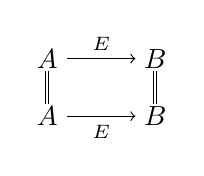
\begin{tikzpicture}[x=1.3em,y=1.3em]
  \node at (0,1.6) {$A$};
  \node at (3.0,1.6) {$B$};
  \node at (0,0) {$A$};
  \node at (3.0,0) {$B$};
  \draw[->] (0.55,1.6) -- (2.45,1.6);
  \node at (1.5,2.02) {$\scriptstyle E$};
  \draw[double,double distance=0.6pt] (0,1.25) -- (0,0.35);
  \draw[double,double distance=0.6pt] (3.0,1.25) -- (3.0,0.35);
  \draw[->] (0.55,0) -- (2.45,0);
  \node at (1.5,-0.45) {$\scriptstyle E$};
\end{tikzpicture}
\qquad $:=$ \qquad
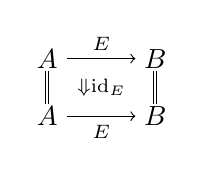
\begin{tikzpicture}[x=1.3em,y=1.3em]
  \node at (0,1.6) {$A$};
  \node at (3.0,1.6) {$B$};
  \node at (0,0) {$A$};
  \node at (3.0,0) {$B$};
  \draw[->] (0.55,1.6) -- (2.45,1.6);
  \node at (1.5,2.02) {$\scriptstyle E$};
  \draw[double,double distance=0.6pt] (0,1.25) -- (0,0.35);
  \draw[double,double distance=0.6pt] (3.0,1.25) -- (3.0,0.35);
  \node at (1.5,0.8) {$\scriptstyle\Downarrow\mathrm{id}_{E}$};
  \draw[->] (0.55,0) -- (2.45,0);
  \node at (1.5,-0.45) {$\scriptstyle E$};
\end{tikzpicture}
\end{center}
\item 竖直边界函子为恒同、从而其源\trSpan{}与目标\trSpan{}都居于同一对
$\oo$-范畴之间的胞腔
\begin{center}
$\mu\colon E_{1}\divideontimes\cdots\divideontimes E_{n}\Rightarrow E$
\qquad $:=$ \qquad
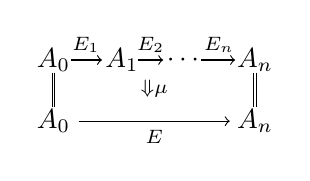
\begin{tikzpicture}[x=1.3em,y=1.3em]
  \node at (0,1.7) {$A_{0}$};
  \node at (1.9,1.7) {$A_{1}$};
  \node at (3.6,1.7) {$\cdots$};
  \node at (5.6,1.7) {$A_{n}$};
  \draw[->] (0.5,1.7) -- (1.35,1.7);
  \node at (0.9,2.12) {$\scriptstyle E_{1}$};
  \draw[->] (2.35,1.7) -- (3.05,1.7);
  \node at (2.7,2.12) {$\scriptstyle E_{2}$};
  \draw[->] (4.1,1.7) -- (5.05,1.7);
  \node at (4.6,2.12) {$\scriptstyle E_{n}$};
  \draw[double,double distance=0.6pt] (0,1.35) -- (0,0.4);
  \draw[double,double distance=0.6pt] (5.6,1.35) -- (5.6,0.4);
  \node at (2.8,0.9) {$\scriptstyle\Downarrow\mu$};
  \node at (0,0) {$A_{0}$};
  \node at (5.6,0) {$A_{n}$};
  \draw[->] (0.7,0) -- (4.9,0);
  \node at (2.8,-0.45) {$\scriptstyle E$};
\end{tikzpicture}
\end{center}
可以用记号 $\mu\colon E_{1}\divideontimes\cdots\divideontimes E_{n}\Rightarrow E$ 排入行内；%
这一表述隐含地断言，定义域中出现的诸\trModule{}定义一个相容序列，其中符号%
「$\divideontimes$」意在暗示 (8.1.9) 中作为水平定义域出现的那个\trPullback{}，而非%
一个\trProduct{}。在模的虚拟装备中，形如
$\mu\colon E_{1}\divideontimes\cdots\divideontimes E_{n}\Rightarrow E$ 的胞腔对应于定义
8.1.1 所引入意义下的\emph{纤维化映射}（fibered maps）。
\item 给定从 $A_{0}$ 到 $A_{n}$ 的一个相容\trModule{}序列
$E_{1}\divideontimes\cdots\divideontimes E_{n}$，我们记
$A_{0}\mathrel{\overset{\vec{E}}{\leftrightsquigarrow}}A_{n}$ 表示复合而成的%
\trTwoSidedFibration{}，并类似地把以该序列为源的一个 $n$ 元\trModule{}映射
(8.1.9) 缩写为如下左图：
\begin{center}
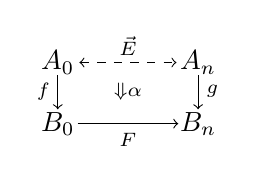
\begin{tikzpicture}[x=1.3em,y=1.3em]
  \node at (0,1.7) {$A_{0}$};
  \node at (3.9,1.7) {$A_{n}$};
  \draw[<->,dashed] (0.6,1.7) -- (3.3,1.7);
  \node at (1.95,2.15) {$\scriptstyle\vec{E}$};
  \draw[->] (0,1.35) -- (0,0.4);
  \node at (-0.4,0.9) {$\scriptstyle f$};
  \draw[->] (3.9,1.35) -- (3.9,0.4);
  \node at (4.3,0.9) {$\scriptstyle g$};
  \node at (1.95,0.9) {$\scriptstyle\Downarrow\alpha$};
  \node at (0,0) {$B_{0}$};
  \node at (3.9,0) {$B_{n}$};
  \draw[->] (0.55,0) -- (3.35,0);
  \node at (1.95,-0.45) {$\scriptstyle F$};
\end{tikzpicture}
\qquad $:=$ \qquad
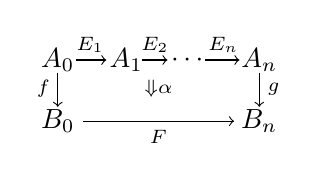
\begin{tikzpicture}[x=1.3em,y=1.3em]
  \node at (0,1.7) {$A_{0}$};
  \node at (1.9,1.7) {$A_{1}$};
  \node at (3.6,1.7) {$\cdots$};
  \node at (5.6,1.7) {$A_{n}$};
  \draw[->] (0.5,1.7) -- (1.35,1.7);
  \node at (0.9,2.12) {$\scriptstyle E_{1}$};
  \draw[->] (2.35,1.7) -- (3.05,1.7);
  \node at (2.7,2.12) {$\scriptstyle E_{2}$};
  \draw[->] (4.1,1.7) -- (5.05,1.7);
  \node at (4.6,2.12) {$\scriptstyle E_{n}$};
  \draw[->] (0,1.35) -- (0,0.4);
  \node at (-0.4,0.9) {$\scriptstyle f$};
  \draw[->] (5.6,1.35) -- (5.6,0.4);
  \node at (6.0,0.9) {$\scriptstyle g$};
  \node at (2.8,0.9) {$\scriptstyle\Downarrow\alpha$};
  \node at (0,0) {$B_{0}$};
  \node at (5.6,0) {$B_{n}$};
  \draw[->] (0.7,0) -- (4.9,0);
  \node at (2.8,-0.45) {$\scriptstyle F$};
\end{tikzpicture}
\end{center}
\end{itemize}
\end{notation}
